\chapter{Tests und Analyse}
\label{cha:Analyse}
Dieses Kapitel beschäftigt sich mit den Tests und der Analyse des implementierten Vorlagenmanagements. Es gibt zwei Arten von Tests die implementiert wurden:
\begin{enumerate}
	\item Die Tests, die nicht auf eine \emph{CDI}-Umgebung angewiesen sind und 
	\item die Tests, die auf eine \emph{CDI}-Umgebung angewiesen sind.
\end{enumerate}

\section{Tests}
\label{sec:Tests}
Dieser Abschnitt beschäftigt sich mit den Tests des Vorlagenmanagements. Für die Tests wurden folgende Bibliotheken verwendet:
\begin{itemize}
	\item\emph{JUnit4} [\cite{junit4}] ist eine Bibliothek, die ein vollwertiges Test-\emph{Framework} darstellt, mit dem wiederholbare und reproduzierbare Tests implementiert werden können.
	\item\emph{DeltaSpike} [\cite{deltaspike}] ist ein Projekt von der \emph{Apache Software Foundation} (\emph{ASF}), das Module bereitstellt, die portable \emph{CDI}-Erweiterungen sind, und auch ein Modul für \emph{JUnit}-Tests in einer \emph{CDI}-Umgebung, basierend auf der Bibliothek \emph{JUnit4}.
	\item\emph{H2} [\cite{h2}] ist eine Bibliothek, mit der eine \emph{In-Memory}-Datenbank erstellt werden kann.  
\end{itemize}
\ \newline
Alle implementierten Tests sind nicht auf einen Anwendungsserver angewiesen und sind in jeder Entwicklungsumgebung wie z.B \emph{Eclipse} oder \emph{IntelliJ} und bei einem Kompilieren über das \emph{Buildtool Maven} ausführbar.
\newline
\newline
Bezüglich der Tests, die in einer \emph{CDI}-Umgebung lauffähig sein müssen, sei auf den  Blogeintrag von [\cite{strubergBlog}] verwiesen, der die Problematik der Nutzung einer \emph{CDI}-Umgebung innerhalb der \emph{Java Standard Edition} (\emph{JSE}) erklärt. Als Lösungsansatz wird ein Modul der Bibliothek von \emph{DeltaSpike} namens \emph{ContainerControl} vorgestellt, das eine einfache Handhabung einer \emph{CDI}-Umgebung ermöglicht und auch bei den folgenden Tests verwendet wird.
\newline
\newline
Die Tests wurden wie folgt organisiert:
\begin{itemize}
	\item\emph{com.clevercure.mailing.test.*} ist das \emph{Java}-Paket, in dem alle implementierten Tests liegen. 
	\item\emph{*.[toTestClass]Tests} ist das \emph{Java}-Paket für eine zu testende Klasse, wobei der Paketname den Namen der zu testenden Klasse mit dem Suffix \grqq Tests\grqq ~ enthält.
	\item\emph{[toTestMethod]Test} ist die Klasse für die Tests einer Methode der zu testenden Klasse.
	\item\emph{test\_case} ist der Name der einzelnen Testmethoden, der angibt, was an einer Methode getestet wird. 
\end{itemize}
\ \newline
Die vorgestellte Konvention der Tests wurde umgesetzt, sofern es möglich war, da es auch Tests gibt, die nicht mit dieser Konvention implementiert werden können.

\subsection{Tests der \emph{CDI}-Integration}
Die Tests aus Abbildung \ref{fig:tests-template-cdi} testen die Implementierungen des Artefakts \emph{mailing-moule-template-cdi}, das die \emph{CDI}-Integration des Variablenmanagements enthält. Es werden die Klassen wie
\begin{itemize}
	\item \emph{TemplateCdiExtension},
	\item \emph{VariableResolverFactoryProvider},
	\item \emph{CdiTemplateUtils} und 
	\item \emph{TemplateResourceProducer}
\end{itemize}
getestet.
\newline
\newline
Diese Tests sind nur lauffähig in einer \emph{CDI}-Umgebung, die mit der Bibliothek \emph{DeltaSpike} im Klassenpfad gestartet werden kann. Im Klassenpfad der Tests wurden Variablen und eine Implementierung der Klasse \emph{VariableResolverFactory} implementiert. Mit diesen Tests wird sichergestellt, dass die \emph{CDI}-Integration des Vorlagenmanagements, aus Sicht der Implementierung, korrekt funktioniert. Diese Tests gewährleisten nicht, dass die \emph{CDI}-Integration in jeder Implementierung einer \emph{CDI}-Umgebung funktioniert, da es hier durchaus Unterschiede geben kann. Um garantieren zu können, dass das Vorlagenmanagement in der verwendeten implementierten \emph{CDI}-Umgebung funktioniert, müssen Integrationstests implementiert werden, die im verwendeten Anwendungsserver ausgeführt werden.
\newpage

\begin{figure}[h]
\centering
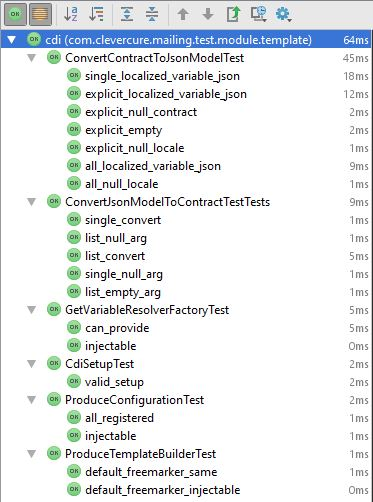
\includegraphics[scale=0.9]{tests-template-cdi}
\caption{Die Tests des Artefakts \emph{mailing-moule-template-cdi}}
\label{fig:tests-template-cdi}
\end{figure}

\subsection{Tests der \emph{JSF}-Integration}
Die Tests aus Abbildung \ref{fig:tests-template-jsf} testen die Implementierungen des Artefakts \emph{mailing-module-template-jsf}, das die \emph{JSF}-Integration des Variablenmanagements enthält. Es wird der implementierte \emph{FacesConverter FreemarkerTemplateConverter} getestet. Obwohl die Klasse \emph{FreemarkerTemplateConverter} innerhalb des \emph{JSF-Framworks} verwendet wird, ist es nicht notwendig, eine \emph{JSF}-Umgebung zu simulieren oder zu starten. Der Konverter greift nicht auf die Formalparameter \emph{UIComponent} und \emph{FacesContext} zu, daher ist es nicht notwendig, \emph{Mocks} für diese Objekte zur Verfügung zu stellen. Diese Tests sind aber auf eine \emph{CDI}-Umgebung angewiesen, da in der Implementierung mit der \emph{CDI}-Umgebung interagiert wird und \emph{CDI-Beans} verwendet werden.

\begin{figure}[h]
\centering
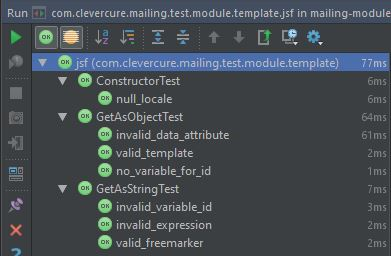
\includegraphics[scale=0.9]{tests-template-jsf}
\caption{Die Tests des Artefakts \emph{mailing-moule-template-jsf}}
\label{fig:tests-template-jsf}
\end{figure}

\subsection{Tests des Vorlagenmanagements}
Die Tests aus Abbildung \ref{fig:tests-template-impl} testen die Implementierungen des Artefakts \emph{mailing-module-template-logic-impl}, welches die Implementierungen des Vorlagenmanagements enthält. Es werden die Klassen \emph{VariableConfigurationImpl} und \emph{FreemarkerTemplateDataJsonBuilder}  getestet.
\newline
\newline
Diese Tests sind nicht abhängig von einer \emph{CDI}-Umgebung und können mit der Bibliothek \emph{JUnit4} alleine getestet werden. Es wird getestet ob Variablen korrekt registriert werden und in einem Objekt der Klasse \emph{VariableConfigurationImpl} korrekt verwaltet werden, und ob die Klasse \emph{FreemarkerTemplateDataJsonBuilder} in der Lage ist, die verschiedenen Repräsentationen des Datenobjekts zu produzieren, das die Daten für eine Voralge hält.
\newline
\newline
Es müssen noch weitere Tests für die beiden Klassen \emph{FreemarkerTemplateProcessor} und \emph{FreemarkerTemplateMetadata} 
implementiert werden.
\newpage

\begin{figure}[h]
\centering
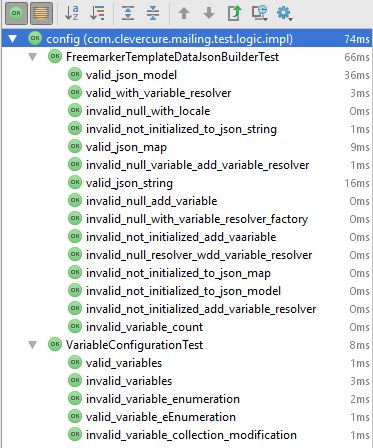
\includegraphics[scale=0.9]{tests-template-impl}
\caption{Die Tests des Artefakts \emph{mailing-moule-template-logic-impl}}
\label{fig:tests-template-impl}
\end{figure}

\section{Analyse}
Dieser Abschnitt beschäftigt sich mit der Analyse der Implementierung des Vorlagenmanagements, dessen Integration in eine \emph{CDI}-Umgebung und \emph{JSF}, sowie der implementierten Beispielwebanwendung. Es wurden alle Anforderung, die im Kapitel \ref{cha:Zielsetzung} vorgegeben wurden, erfüllt.

\subsection{\emph{CKEditor-Plugin} des Vorlagenmanagements}
Es wurde erfolgreich ein \emph{Plugin} für den \emph{CKEditor} implementiert, sowie ein Variablenmanagement für die \emph{Browser}-seitige Verwaltung der Variablen. Wie in Abschnitt \ref{sec:sub-typescript-javascript} vorgegeben, wurde das \emph{CKEditor-Plugin} und das Variablenmanagement in \emph{TypeScript} getrennt voneinander in eigenen Quelltextdateien implementiert. Die \emph{TypeScript}-Quelltexte befinden sich zurzeit noch in der Beispielwebanwendung, da die Entwicklung in einem eigenen Projekt nicht möglich war, da das \emph{Hot Code Deployment} für \emph{Java}-Ressourcen (\emph{src/main/resources}) nicht unterstützt wird. Die Quelltextdateien können einfach in ein anderes Projekt verschoben werden. Die \emph{TypeScript}-Quelltexte werden jetzt noch über die Entwicklungsumgebung kompiliert. In Zukunft müssen die \emph{TypeScript}-Quelltexte mit dem \emph{Buildtool Maven} über das \emph{Maven Build Plugin maven-grunt-plugin} automatisiert bei jedem \emph{Maven-Build} kompiliert werden.

\subsection{\emph{CDI}-Integration des Vorlagenmanagements}
Es wurde erfolgreich die Integration des Vorlagenmanagement in eine \emph{CDI}-Umgebung implementiert. Die in Abschnitt \ref{sec:sub-impl-integartion-cdi} behandelte Integration in eine \emph{CDI}-Umgebung, wurde über eine portierbare \emph{CDI}-Erweiterung realisiert. Als nächster Schritt könnten auch Variablen unterstützt werden, die nicht über einen eigenen Aufzählungstyp definiert werden. Dazu müsste die Methode \emph{processCdiVariableContracts} der Klasse \emph{TemplateCdiExtension} und die Klasse \emph{VariableConfigurationImpl} erweitert werden. Die Klasse \emph{TemplateCdiExtension} müsste die registrierten Typen der Schnittstelle \emph{VariableContract} in einem Behälter verwalten und die Klasse \emph{VariableConfigurationImpl} müsste in der Lage sein, die registrierten Variablen dynamisch aus einer \emph{CDI}-Umgebung zu holen. Es müsste eine Schnittstelle eingeführt werden, die das Holen der Variablen aus der \emph{CDI}-Umgebung für die Klasse \emph{VariableConfigurationImpl} abstrahiert, damit es keine Abhängigkeiten zu Klassen von \emph{CDI} gibt.

\subsection{\emph{JSF}-Integration des Vorlagenmanagements}
Es wurde erfolgreich eine Integration in \emph{JSF} implementiert, wobei diese Integration über den implementierten \emph{FacesConverter} \emph{FreemarkerTemplateConverter} erreicht wurde, der die Vorlagen von ihrer \emph{HTML}-Repräsentation in die \emph{Freemarker}-Repräsentation konvertieren kann. Wie in Abschnitt \ref{sec:sub-impl-integartion-jsf} vorgestellt, wurde die gemeinsame Logik in einer abstrakten Klasse \emph{AbstractTemplateConverter} gekapselt, der nur bekanntgegeben werden muss, welche konkrete Implementierung, definiert über ein Annotationsliteral für den Qualifizierer, genutzt werden soll. Wenn man auf \emph{JSF 2.3} wechselt, könnte man die dynamische Interaktion mit der \emph{CDI}-Umgebung durch statische Injektionspunkte ersetzten, die auch beim Start der \emph{CDI}-Umgebung validiert werden. 
\newline
\newline
Dieses Kapitel beschäftigte sich mit den Tests und der Analyse der Implementierungen und der Integration des Vorlagenmanagements. Das nächste Kapitel \ref{cha:Zusammenfassung} befasst sich mit der Zusammenfassung, mit den weiteren Aufgaben, und den gemachten Erfahrungen.